\chapter{Darstellung der DICOM-Elemente im Speicher} \label{appendix:speicher}
\section{Explizite VR mit [ OB \textpipe\ OW \textpipe\ OF \textpipe\ SQ \textpipe\ UT \textpipe\ UN ]}

Bei expliziter VR-Struktur besteht das Element aus vier konsekutiven Feldern. Ist die VR vom Typ OB, OW, OF, SQ, UT oder UN wird das Datenelement wie in Tabelle \ref{table:appendix_explizit} im Speicher abgelegt. Die reservierten 2 Byte im VR-Teil sind für zukünftige Weiterentwicklungen des DICOM-Standards.\cite[7.1.2]{dicom:structure}

\begin{sidewaystable}
    \begin{tabularx}{\textwidth}{|X|X|p{5cm}|X|X|p{8cm}|}
    \toprule \hline
   \multicolumn{2}{|l|}{\textbf{Tag}} 	&	\multicolumn{2}{l|}{\textbf{VR}} 		&		\textbf{Value Length}   	& 	\textbf{Value} \\ \hline
    Group \# 16-bit unsigned integer & Element \# 16-bit unsigned integer  &  VR 2-byte character String [OB | OW | OF | SQ | UT | UN ] & Reservierter
    Bereich & 32-bit unsigned integer  &  Gerade Anzahl an Byte. Enthält den Wert des Datenelements. Kodierung abhängig von VT-Typ und Transfersyntax. Wenn die Länge nicht definiert ist wird diese auf \glqq Sequence Delimitation\grqq\ limitiert. \\ \hline
	
	2 Byte & 2 Byte & 2 Byte & 2 Byte & 4 Byte & Anzahl an Byte entsprechend der \glqq Value Length\grqq\, wenn von explizieter Länge \\ \hline
	
	\bottomrule
    \end{tabularx}
    \caption {Darstellung des Datenelements im Speicher wenn VR vom Typ OB, OW, OF, SQ, UT oder UN}
    \label{table:appendix_explizit}
\end{sidewaystable}

\section{Explizite VR}

Diese Darstellung wird gewählt wenn VR \textit{nicht} vom Typ OB, OW, OF, SQ, UT oder UN ist. Der Unterschied besteht im Feld \glqq Value Length\grqq\. Bei der Form von Tabelle \ref{table:appendix_explizit} ist dieses Feld 32 Bit lange. Hier beträgt es lediglich 16 Bit \cite[7.1.2]{dicom:structure}. Der Grund liegt am erhöhten Speicherbedarf von \ref{table:appendix_explizit}, da die Länge des Wertes eine undefinierte Länge haben kann.

\begin{sidewaystable}
	\begin{tabularx}{\textwidth}{|X|X|X|X|p{12cm}|}
	\toprule \hline
	\multicolumn{2}{|l|}{\textbf{Tag}} & \textbf{VR} 2 & \textbf{Value Length} & \textbf{Value} 4 \\ \hline
	Group \# 16-bit unsigned integer & Element \# 16-bit unsigned integer & VR 2-byte character String 2 & 16-bit unsigned integer & Gerade Anzahl an Byte. Enthält den Wert des Datenelements. Kodierung abhängig von VT-Typ und Transfersyntax. \\ \hline
	2 Byte & 2 Byte & 2 Byte & 2 Byte & \glqq Value Length\grqq\ Byte \\ \hline
	\bottomrule
	\end{tabularx}
    \caption {Darstellung des Datenelements für alle anderen VR-Typen}
    \label{table:appendix_explizit_else}
\end{sidewaystable}

\section{Implizite VR}

Bei einer impliziten VR Darstellung besteht das Datenelement aus den drei konsekutive Feldern Tag, Value Length und dem Wert selbst \cite[7.1.3]{dicom:structure}.

\begin{sidewaystable}
	\begin{tabularx}{\textwidth}{|X|X|X|p{12cm}|}
	\toprule \hline
	\multicolumn{2}{|l|}{\textbf{Tag}} & \textbf{Value Length} 2 & \textbf{Value} \\ \hline
	Group \# 16-bit unsigned integer & Element \# 16-bit unsigned integer & 32-bit unsigned integer & Gerade Anzahl an Byte. Enthält den Wert des Datenelements. Kodierung abhängig von VT-Typ spezifiziert in \cite{dicom:dd} und Transfersyntax. Wenn die Länge nicht definiert ist wird diese auf \glqq Sequence Delimitation\grqq\ limitiert. \\ \hline
	2 Byte & 2 Byte & 2 Byte & \glqq Value Length\grqq\ Byte oder undefinierte Länge \\ \hline
	
	\bottomrule
	
	\end{tabularx}
    \caption {Darstellung des Datenelements für implizite VR.}
    \label{table:appendix_implizit}
\end{sidewaystable}


\chapter{Installation der Eclipse e4 Umgebung}

\section{Eclipse}
Voraussetzung für Eclipse ist eine bereits installierte Java Virtual Machine. Werden keine Werkzeuge aus dem Java Development Kit benötigt, reicht eine Java Runtime Environment aus.
Grundlage für die Plug-in und Rich Client Entwicklung ist eine Eclipse-Installation. Unter \textit{http://www.eclipse.org/downloads/} kann der aktuelle \textit{Eclipse Standard Client} für ein beliebiges Betriebssystem bezogen werden. Bei der Wahl zwischen 32- und 64-Bit muss die Version mit der installierten Java-Variante übereinstimmen, da sonst die Native Libraries nicht geladen werden können. Nach dem Entpacken des Zip-Archivs kann der Client über \textit{eclipse.exe} werden. Abbildung \ref{eclipsestd} zeigt das Programmfenster von Eclipse nach dem ersten Ausführen.\\

\begin{figure}[H]
  \vspace{0.5cm}
  \centering
  \fbox{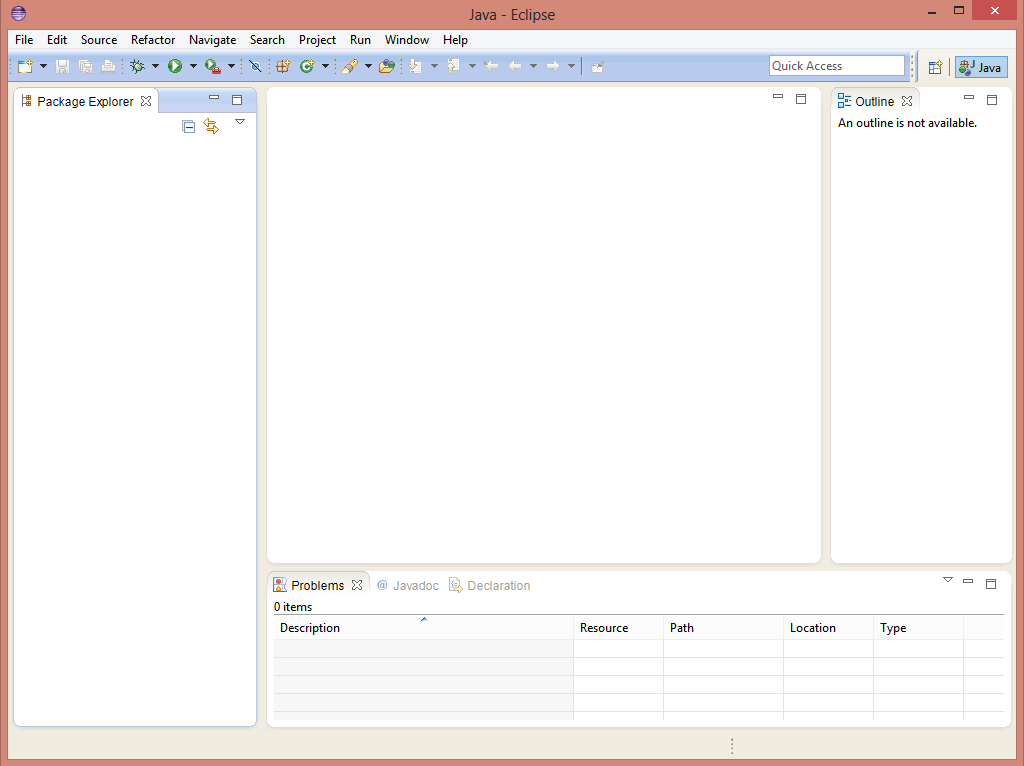
\includegraphics[angle=0,width=8cm]{./img/eclipse_std.png}}
  \caption{Standardinstallation eines 32-Bit Eclipse unter Windows 8}
  \label{eclipsestd}
  \vspace{0.5cm}
\end{figure}

\section{Eclipse e4 Tools}
Eine weitere Voraussetzung ist eine Installation der e4 Tools. Das e4 Projekt ist unter \textit{http://download.eclipse.org/e4/downloads/} mit dem Punkt \textit{Stable Build} zu finden (Abbildung \ref{e4download}). 

\begin{figure}[H]
  \vspace{0.5cm}
  \centering
  \fbox{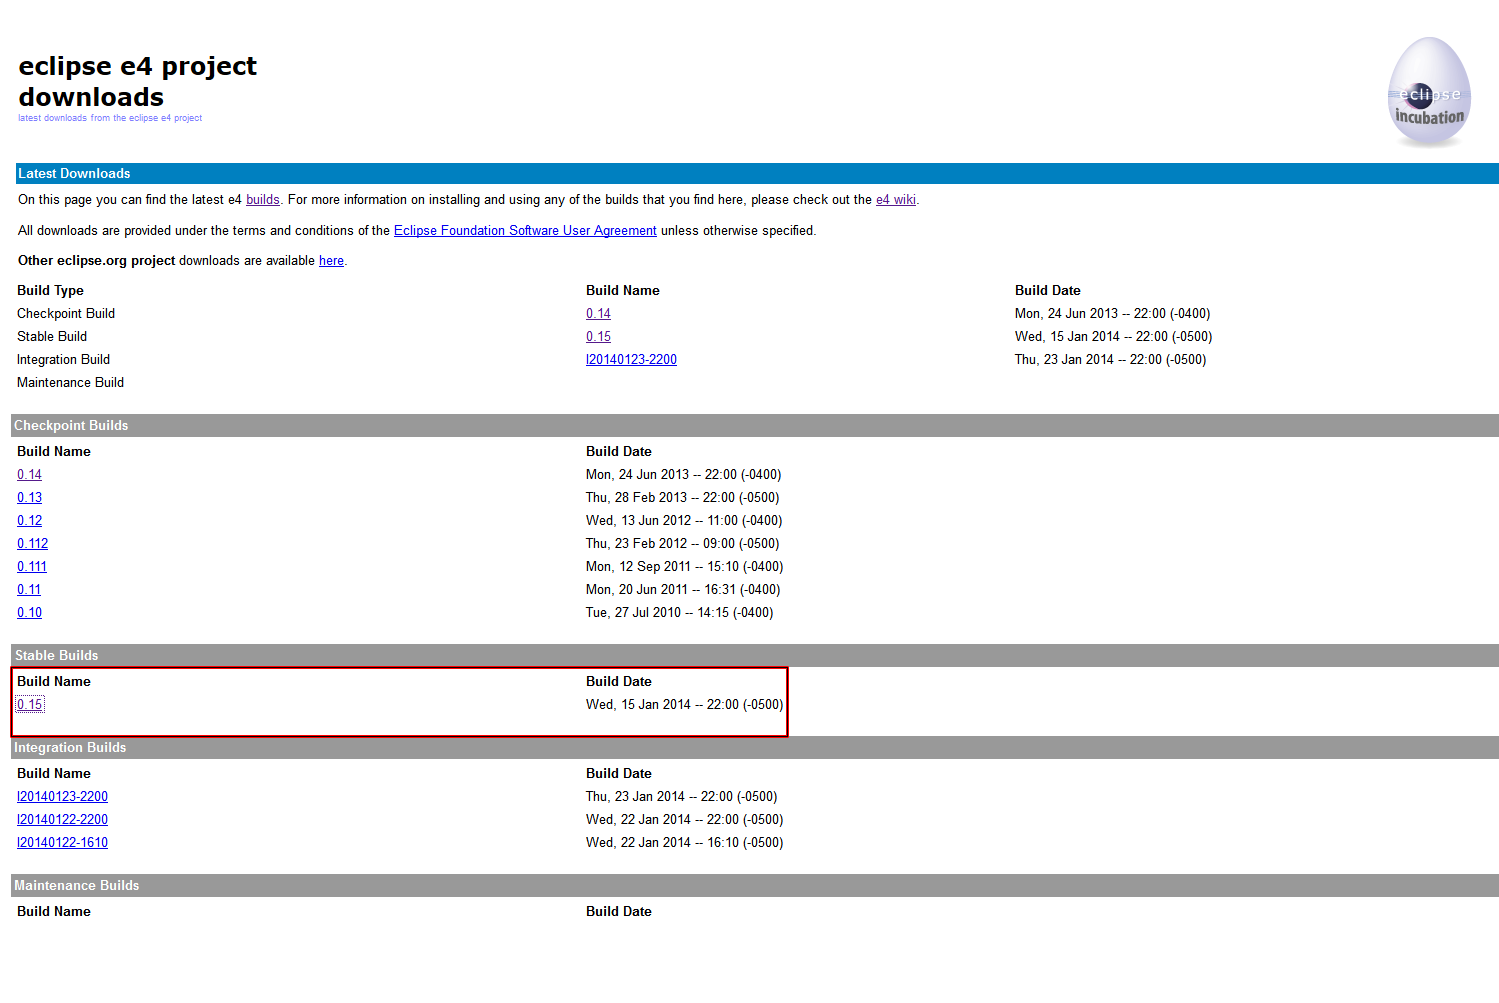
\includegraphics[angle=0,width=8cm]{./img/e4download.png}}
  \caption{e4 Projekt Builds}
  \label{e4download}
  \vspace{0.5cm}
\end{figure}

Nach einem Klick auf den aktuellen Build öffnet sich die Seite mit dem Link zum Repository wie in Abbildung \ref{repolink} rot markiert.\\
Dieser Link (\textit{http://download.eclipse.org/ e4/ downloads/ drops/ S-0.15-201401152200/ repository} - Stand 24.01.2014) muss nun in die Zwischenablage kopiert werden.

\begin{figure}[H]
  \vspace{0.5cm}
  \centering
  \fbox{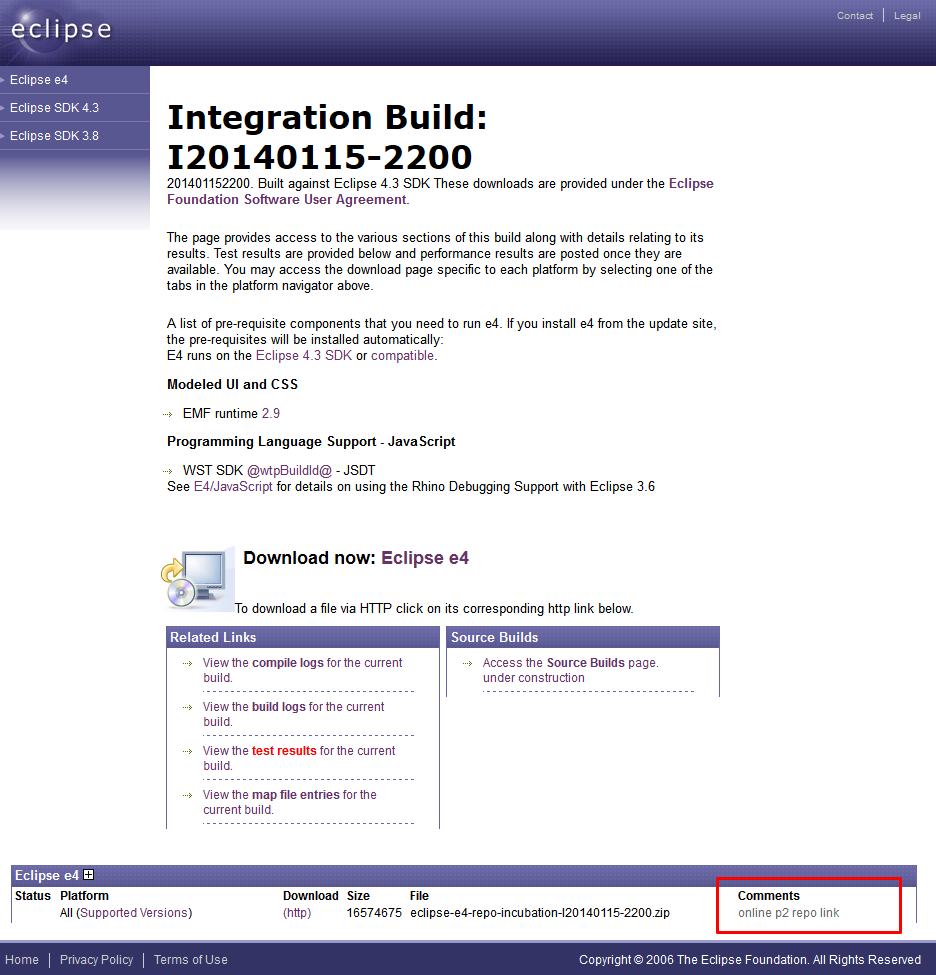
\includegraphics[angle=0,width=8cm]{./img/repolink.png}}
  \caption{e4 Repository Link}
  \label{repolink}
  \vspace{0.5cm}
\end{figure}

Nachdem der Link kopiert wurde, kann Eclipse geöffnet werden. Nach einem Klick auf den Menüpunkt \textit{Hilfe} $\rightarrow$ \textit{Install New Software} öffnet sich ein Fenster mit dem Titel \glqq Available Software\grqq\ wie in Abbildung \ref{installnew} zu sehen ist. 

\begin{figure}[H]
  \vspace{0.5cm}
  \centering
  \fbox{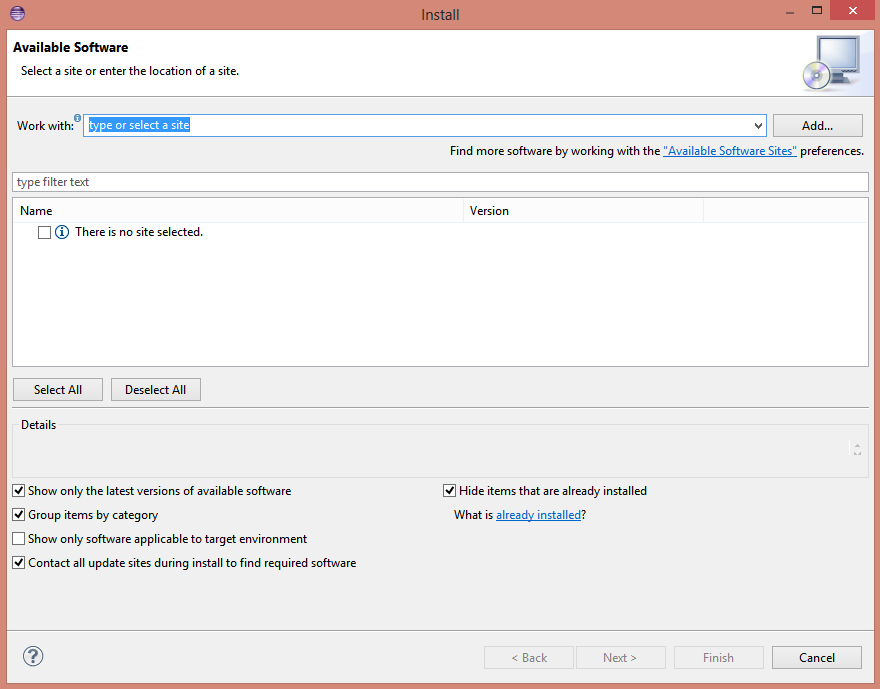
\includegraphics[angle=0,width=8cm]{./img/installnew.png}}
  \caption{Installation neuer Software unter Eclipse}
  \label{installnew}
  \vspace{0.5cm}
\end{figure}

Mit dem Button \textit{Add} muss nun der zuvor kopierte Links als Repository angegeben werden. Der \textit{Name} kann frei vergeben werden und unter \textit{Location} muss der Link zum Repository eingetragen werden. Danach mittels \textit{OK} die Aktion bestätigen.

\begin{figure}[H]
  \vspace{0.5cm}
  \centering
  \fbox{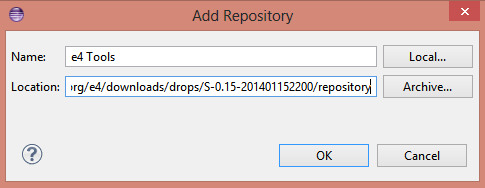
\includegraphics[angle=0,width=6cm]{./img/insertrepo.png}}
  \caption{Angabe des Repository}
  \label{insertrepo}
  \vspace{0.5cm}
\end{figure}

Nach einem korrekten Eintrag wird die Liste der verfügbaren Software, wie in Abbildung \ref{e4install} zu sehen ist, aktualisiert. Hier muss das Paket \textit{Eclipse 4 core tools} samt Unterpakete ausgewählt werden. Mit einem Klick auf \textit{Next} startet die Installationsroutine. Hierbei den Anweisungen auf dem Bildschirm folgen. Nach einer erfolgreichen Installation muss Eclipse neu gestartet werden.

\begin{figure}[H]
  \vspace{0.5cm}
  \centering
  \fbox{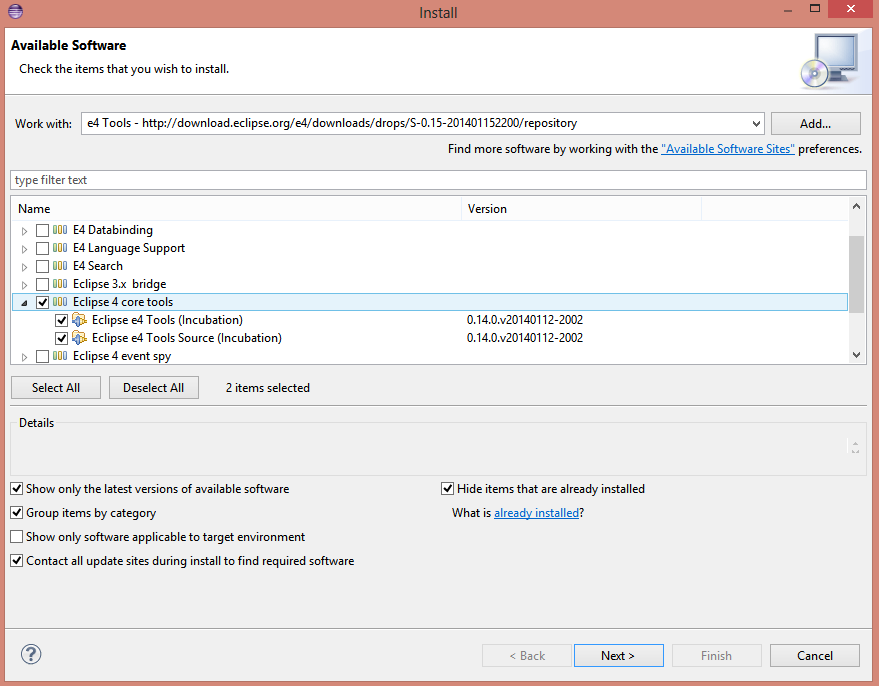
\includegraphics[angle=0,width=8cm]{./img/e4install.png}}
  \caption{Auswahl der e4 Tools zur Installation}
  \label{e4install}
  \vspace{0.5cm}
\end{figure}

\section{Import der jMediKit Projektdateien}

Die Projektdaten befinden sich als auf dem beiliegenden Datenträger. Das Wurzelverzeichnis kann als Eclipse Workspace benutzt werden. Dabei ist darauf zu achten, dass der Ordner \textit{/.metadata/.plugins} leer ist. Sollten sich Daten darin befinden, können diese gelöscht werden. Eclipse erstellt bei Bedarf die Plug-in-Daten neu. Der Workspace besteht aus den drei Projekten \textit{org.jmedikit.product}, \textit{org.jmedikit.feature} und \textit{org.jmedikit.plugin}. Beim ersten Öffnen ist der Package Explorer leer und die Projekte müssen importiert werden. Nach einem Klick auf \textit{File} $\rightarrow$ \textit{Import} erscheint ein Dialog wie in Abbildung \ref{importproject} zu sehen ist. Bei der Auswahl muss der Punkt unter \textit{General} $\rightarrow$ \textit{Existing Projects into Workspace} markiert und mit \textit{Next} bestätigt werden. Im folgenden Fenster (Abbildung \ref{selectimport}) muss unter ausgewähltem \textit{Select Root Directory} unter \textit{Browse} das Wurzelverzeichnis von jMediKit angegeben werde. Danach können die verfügbaren Projekte hinzugefügt und mittels Klick auf \textit{Finish} in den Eclipse Workspace importiert werden.

\begin{figure}[H]
%\subfigure[Keypoints]{\includegraphics[width=0.49\textwidth]{./img/basmati_keypoints.png}}\hfill
\centering
\fbox{
\subfigure[Dialog zum Import von Eclipse-Projekten]{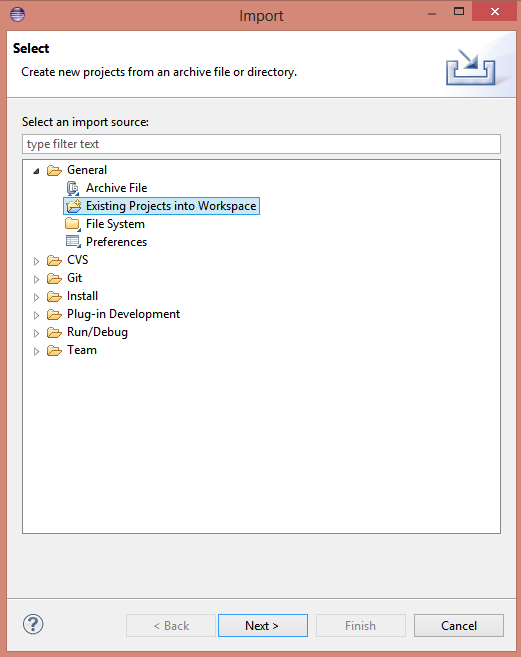
\includegraphics[width=6cm]{./img/import.png} \label{importproject}}
\subfigure[Auswahl der Projekte]{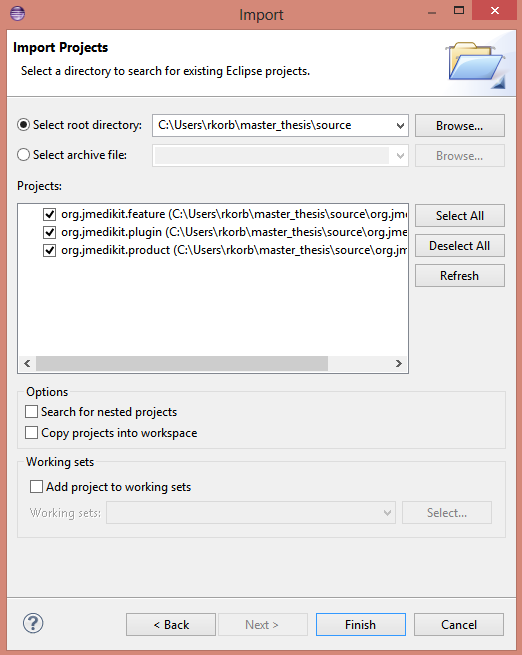
\includegraphics[width=6cm]{./img/importprojects.png} \label{selectimport}}
}
\caption{Vorgang zum Importieren bereits bestehender Projekte}
\label{import}
\end{figure}

War der Importvorgang erfolgreich, sind die drei Projekte 

\begin{itemize}
\item \textit{org.jmedikit.product}
\item \textit{org.jmedikit.feature}
\item  \textit{org.jmedikit.plugin} 
\end{itemize}

wie in Abbildung \ref{finishedimport} zu sehen, im Package Explorer vorhanden.

\begin{figure}[H]
  \vspace{0.5cm}
  \centering
  \fbox{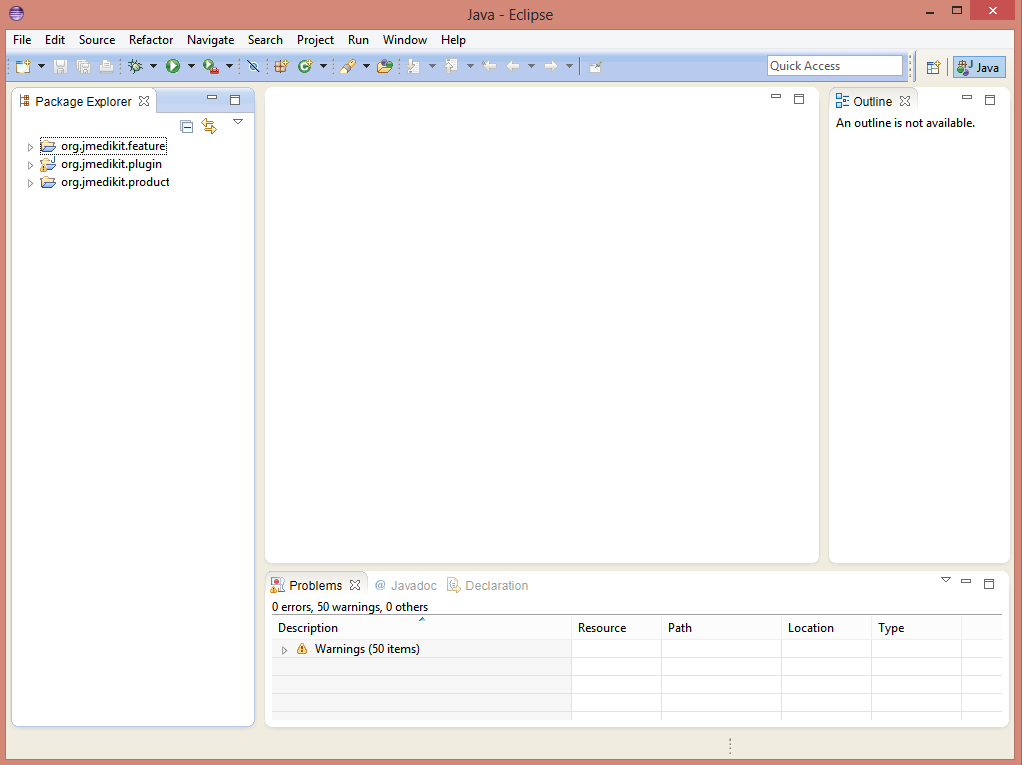
\includegraphics[angle=0,width=8cm]{./img/imported.png}}
  \caption{Der Package Explorer nach dem Importvorgang}
  \label{finishedimport}
  \vspace{0.5cm}
\end{figure}

Im Projekt \textit{org.jmedikit.product} befindet sich die Datei \textit{jmedikit.product}. Nach einem Doppelklick wird die Datei im Eclipse-Editor geöffnet und zeigt die Grundlegende Anwedungsdefinition von jMediKit und den zugehörigen Einstellungen. Unter dem Tab \textit{Overview} im Bereich \textit{Test} kann jMediKit mit einem Klick auf \textit{Launch an Eclipse application} gestartet werden. Abbildung \ref{launchjmedikit} hebt die Schaltfläche hervor. Bei einem ersten Start wird jMediKit mit einer Fehlermeldung geschlossen, da von Eclipse noch nicht alle zum Start notwendigen Plug-ins geladen wurden, welche von der jMediKit benötigt werden.

\begin{figure}[H]
  \vspace{0.5cm}
  \centering
  \fbox{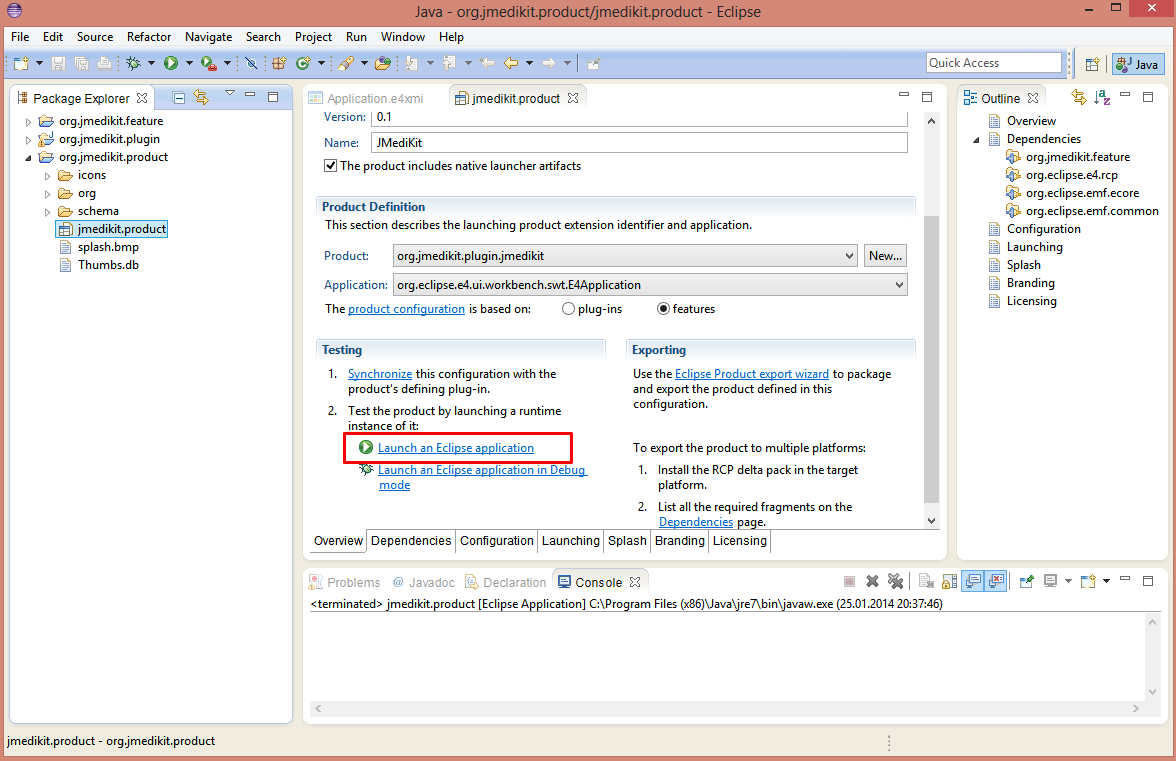
\includegraphics[angle=0,width=8cm]{./img/launch.png}}
  \caption{Der Package Explorer nach dem Importvorgang}
  \label{launchjmedikit}
  \vspace{0.5cm}
\end{figure}

Unter \textit{Run} $\rightarrow$ \textit{Run Configuration} können die Plug-ins zur Verfügung gestellt werden. Abbildung \ref{addplugins} zeigt das Konfigurationsfenster. Im linken Teil muss die Product-Datei jmedikit.product ausgewählt sein. Unter dem Tab \textit{Plug-ins} befindet sich auf der rechten Seite die Schaltfläche \textit{Add Required Plug-ins}. Nach einem Klick auf \textit{Apply} gefolgt von \textit{Run} kann jMediKit gestartet werden.

\begin{figure}[H]
  \vspace{0.5cm}
  \centering
  \fbox{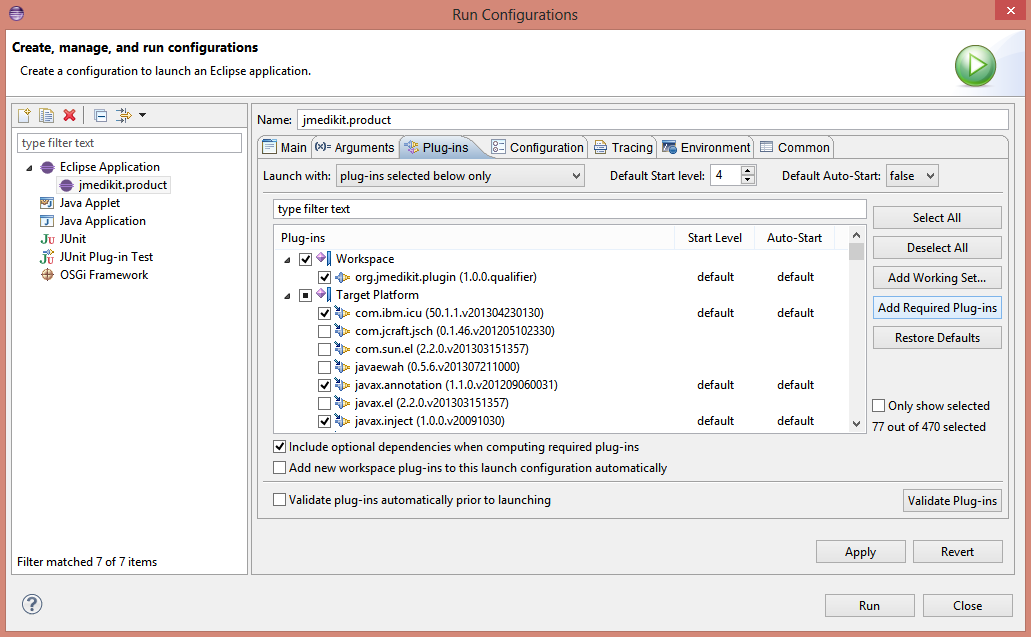
\includegraphics[angle=0,width=8cm]{./img/addplugins.png}}
  \caption{Konfigurationsfenster zu Anwendungseinstellungen und Anwendungsstart}
  \label{addplugins}
  \vspace{0.5cm}
\end{figure}